\subsection{Paleo-Dip}\label{paleo-dip}

It is not possible to assign a \acf{psl} directly from the lava flows as it is with \acf{paz}. However, in the following discussion it will become clear that calculated 3D deformation $D$ depends on all four variables: $\theta,\varphi,\theta',\varphi'$ which completely define each of the initial and final surface attitudes. However, this calculation can be reframed as an optimization problem to obtain constraints on $D$ and $\varphi'$ simultaneously.

The strategy for solving this problem is as follows. First, each surface attitude is interpreted as a unit normal vector expressed in 3D polar coordinates. Since all normal vectors are of unit length, surfaces are interpreted as points on the surface of a sphere, which will prove to be a useful model. The dip of a surface is equal to the colatitude of its normal vector; the dip direction of a surface is equal to the longitude of its normal vector. Since both dip and dip direction are known for the modern (final) surface at each point, the surface attitude is represented by a point on the imaginary unit sphere. Since only dip direction is known of the paleosurface of lava flow/channel emplacement, the range of possible surfaces is represented by an entire line of longitude on the unit sphere. In light of this model, 3D deformation $D$ between two surface attitudes is defined as the (great-circle) distance between their respective point representations on the unit sphere.

Some point withing the line of longitude representing the family of possible paleo-dip values represents the true dip, dip-direction pair at the time of flow emplacement. Which point along this line minimizes the angular distance between the (paleosurface) line and the (modern surface) point? In other words, what paleo-dip $\varphi'$ minimizes total 3D deformation $D$?

This problem is trivial in 2D cartesian coordinates, so the following section outlines the mathematical procedure used to convert the spherical polar case into a planar cartesian analog that retains the key properties of the problem. In particular, the spherical surface should be projected onto a plane such that shortest-paths are preserved; great circle arcs should map to straight lines. The gnomonic projection has this property. See Figure~\ref{gnomonic}.

\def\projectfigsize{5}
\begin{figure}
{\centering
    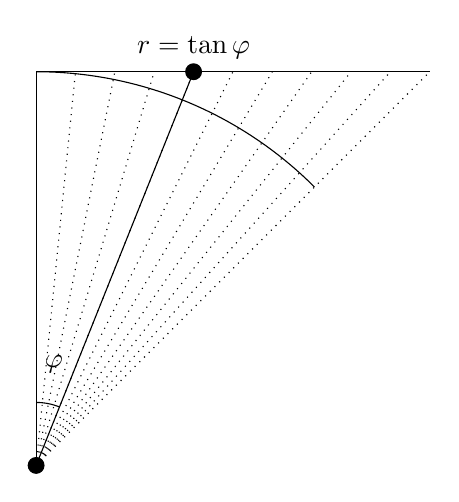
\begin{tikzpicture}
        \draw (45:\projectfigsize) arc (45:90:\projectfigsize);
        \draw (0,\projectfigsize) -- (\projectfigsize,\projectfigsize);
        \filldraw (0,0) circle (.1);
        \filldraw (2,5) circle (.1);
        \foreach \x in {0,0.5,...,\projectfigsize}
            \draw[dotted] (0,0) -- (\x,\projectfigsize);
        \draw (0,0) -- (0,\projectfigsize); 
        \draw (0,0) -- (2,\projectfigsize);
        \draw (90:.8) arc (90:68.19:.8);
        \path +(80:1.3) node {$\varphi$};
        \path +(2,5.3) node {$r=\tan \varphi$};
    \end{tikzpicture}
    \includegraphics[width=0.5\textwidth]{gnomonic.png}
    \caption[Gnomonic projection]{The gnomonic projection maps dip direction (longtitude of normal vector) and dip (colatitude of normal vector) into polar coordinates $r$ and $\theta$. Left: A cross-section along a single line of longtitude $\theta$ is displayed. ($\theta$ does not change during the projection so no new variable is introduced.) Right: Great-circles are mapped to straight lines because a) all great circles are coplanar with the sphere's center, and b) any two non-parallel planes intersect at a line~\parencite{marozols_gnomonic_2022}.}
    \label{gnomonic}
}
\end{figure}

The procedure to solve for $\varphi'$ follows. First, note that the gnomonic projection does not affect longitude $\theta$, so the same variable symbol is used in 3D and 2D polar coordinates. Thus the line\footnote{This line is really a ray from the origin, because any negative values of $r$ for a given $\theta$ in polar coordinates will correspond to a negative slope, which would have been captured by a positive slope for the opposite aspect. This case will be handled later.} of longitude corresponding to the paleo-dip direction does not change when projected into 2D polar coordinates, so no new variable is introduced. In 2D cartesian coordinates, this line has the form:

\begin{equation}
    y=x\cot \theta'.\label{line}
\end{equation}

The point corresponding to the modern surface in polar coordinates:

\begin{equation}
    [r,\theta] = [\tan \varphi, \theta].
\end{equation}

In cartesian coordinates:

\begin{equation}
    [x,y]=[\tan\varphi\sin\theta,\tan\varphi\cos\theta].\label{point}
\end{equation}

The shortest path (minimum 3D deformation $D$) between the line and the point is perpendicular to the line with slope $m=\cot \theta'$, i.e., it has slope $m=-\tan \theta'$. The point-slope form of the perpendicular line is:
\begin{equation}
    y-\underbrace{\tan\varphi\cos\theta}_{y_1}=\underbrace{-\tan \theta'}_{m}(x-\underbrace{\tan\varphi\sin\theta}_{x_1}).\label{perp}
\end{equation}
The intersection point satisfies both~\ref{line} and~\ref{perp}. Substituting from~\ref{line} to find the $x$-coordinate of the intersection point: 
\begin{gather}
    [x\cot \theta']-\tan\varphi\cos\theta=-\tan \theta'(x-\tan\varphi\sin\theta)\nonumber\\
    x\cot \theta'+x\tan \theta'=\tan \theta'\tan\varphi\sin\theta+\tan\varphi\cos\theta\nonumber\\
    x=\frac{\tan\varphi(\cos\theta+\tan\theta'\sin\theta)}{\cot\theta'+\tan\theta'}\nonumber\\
    \boxed{x=\tan\varphi(\cos\theta+\tan\theta'\sin\theta)\sin(2\theta')/2.}\label{x}
\end{gather}
From there, the $y-$coordinate of the intersection point is found by substituting $x$ back into~\eqref{line}. The 2D polar coordinate $r$ is given by $\sqrt{x^2+y^2}$ which is reprojected back onto the sphere (inverse of original gnomonic projection), giving the paleo-dip as desired:
\begin{equation}
    \varphi'=\arctan\sqrt{x^2+y^2}.
\end{equation}
\subsection{Horizontal Deformation}
Before proceeding, we should check that the horizontal deformation  $D_h \equiv |\theta-\theta'|$ does not exceed \ang{90}. If it does, then the previous calculation has produced the nearest uphill slope, rather than the nearest downhill slope, which is not desired. Therefore, any points with such horizontal deformations have their paleo-dip directions redefined to zero. Recall that horizontal deformation is the variable observed by \textcite{chadwick_late_2015,mouginis-mark_late-stage_2019}.
\subsection{3D Deformation}
The angular distance between two normal vectors (equivalently, the dihedral angle between the two surface planes) defines the 3D deformation for each point. Of course, this definition has already been used to construct the mathematical formulation of the paleo-dip constraint, but here the explicit formula for great-circle distance on a unit sphere is used:\footnote{The trigonometric functions cos and sin are swapped for $\varphi$ and $\varphi'$ because these are colatitudes, not latitudes.}
\begin{equation}
    \arccos\left[\cos\varphi\cos\varphi'+\sin\varphi\sin\varphi'\cos(\theta-\theta')\right].
\end{equation}
Recall that this is a minimum constraint, since the paleo-dip used to calculate this value was itself derived using the assumption that $D$ was minimized.